\let\textcircled=\pgftextcircled
\chapter{Background}
\label{chap:background}

\initial{D}\textit{ans ce chapitre nous introduisons ou rappelons les informations et concepts de base nécessaires à la compréhension du travail présenté dans ce document. Il s'agit des notions de \textbf{virtualisation, working set, PML.}}\\
\par

\minitoc

\newpage    
%%%%%%%%%%%%%%%%%%%%%%%%%SECTION VIRTUALISATION%%%%%%%%%%%%%%%%%%%%%%%%%%%%%%%%%%%%%%%%%%%%%%%%%%%%%%%%%
\section{Virtualisation}

\subsection{Généralités}

\subsubsection{Définition}
\par\noindent La virtualisation est l’ensemble des techniques matérielles ou logicielles qui permettent de faire fonctionner simultanément sur une seule machine physique (machine hôte) plusieurs \ac{OS} (\textit{systèmes d’exploitation en français}) appelés \ac{VMs} -\textit{Virtual Machines, en anglais}-.\\

\par\noindent La plupart des serveurs (non virtualisés) utilisent moins de 15\% de leurs capacités \cite{online1}, ce qui favorise leur prolifération et la complexité de leur gestion. La virtualisation résout ces problèmes d’efficacité en permettant l'exécution de plusieurs systèmes d’exploitation sur un même serveur physique sous la forme de machines virtuelles, dont chacune peut accéder aux ressources de calcul du serveur sous-jacent. Chaque VM est une entité isolée, autonome et complètement indépendante des autres. Dans ces environnements virtualisés, un système de virtualisation, \ac{VMM}, est responsable de la gestion de ces machines virtuelles et du partage des ressources entre elles. Il émule le matériel pour elles, et établit la communication entre elles et les périphériques (de la machine hôte). Il existe plusieurs types de systèmes de virtualisation.

\subsubsection{Systèmes de virtualisation}
Le tableau suivant (\ref{tab:sytemes_virtualisation}) présente certaines \acs{VMM}s en fonction de leur type de licence :
\begin{table}[H]
  \begin{center}
    \caption{Systèmes de virtualisation en fonction du type de licence}
    \begin{tabular}{>{\bfseries}l r}
      \hline
      \textbf{VMM} & \textbf{Licence} \\
      \hline
      Bosch & Open source \\ 
      KVM & Open source \\ 
      LXC & Open source \\ 
      Microsoft Virtual PC & Commerciale \\ 
      Parallels & Commerciale \\
      QEMU & Open source \\ 
      VMWare Vcenter & Commerciale \\ 
      VMWare Workstation par nœud & Gratuite (mais pas open source) \\ 
      VNUML (Virtual Network User Model Linux) & Open source \\
      VServer & Open source \\ 
      XEN & Open source \\ \hline
    \end{tabular}
    \label{tab:sytemes_virtualisation}
  \end{center}
\end{table}

Le système que nous utilisons dans le cadre de ce travail est \textbf{XEN}. XEN est un système de virtualisation assez connu \cite{article2} et utilisé par Amazon pour virtualiser ses datacenters \cite{online3}. Il s'appuie sur un hyperviseur qui s'exécute sur le matériel et une achine virtuelle particulière appelée \textit{\textbf{dom0}} : il s'agit de l'OS de la machine hôte. Les services de l'OS hôte ne sont pas inclus dans l'hyperviseur afin de la maintenir aussi léger que possible. Les autres VMs ici sont appelées \textit{\textbf{domU}}.\\
Les systèmes de virtualisation peuvent également être classés en fonction du type de virtualisation qu'elles peuvent exécuter.

\subsubsection{Techniques de virtualisation}
En fonction de la position du système de virtualisation et des machines virtuelles par rapport au matériel, il existe cinq techniques de virtualisation:
\begin{enumerate}[label=\textbf{(\roman*)}]
    \item \textbf{Virtualisation niveau OS} ou \textbf{isolation}. Cette technique de virtualisation permet d'isoler l'exécution des applications des zones d'exécution appelées contextes ou containers. Ici, l'\acs{OS} hôte dispose des mécanismes pour construire des containers isolés (VMs). Ces derniers partagent le même OS (l'hôte). La \acs{VMM} fait donc partie de l'OS hôte. Cette solution est très bonne en performance, mais les environnements virtualisés ne sont pas complètement isolés. La figure \ref{fig:virtualisation_niveau_os} présente l'architecture de cette technique de virtualisation.
    \\ \textbf{Exemples :} OpenVZ,  BSD Jail, chroot, Linux-VServer, Linux containers.
    %\begin{figure}[htp]
    %  \centering
    %  \includegraphics{images/virtualisation_niveau_os.png}
    %  \caption{Architecture Virtualisation niveau OS}
    %  \label{fig:virtualisation_niveau_os}
    %\end{figure}
    
    \item \textbf{Noyau en espace utilisateur}. Un noyau en espace utilisateur (user-space) tourne comme une application en espace utilisateur de l'OS hôte. Le noyau user-space a donc son propre espace utilisateur dans lequel il contrôle ses applications. Cette solution est très peu performante, car deux noyaux sont empilés, l’isolation des environnements n’est pas gérée et l’indépendance par rapport au système hôte est inexistante. Elle sert surtout au développement du noyau. La figure \ref{fig:noyau_espace_utilisateur} présente l'architecture de cette technique de virtualisation.
    \\ \textbf{Exemples :} User Mode Linux, Cooperative Linux, Adeos, L4Linux.
    %\begin{figure}[htp]
    %  \centering
    %  \includegraphics{images/noyau_espace_utilisateur.png}
    %  \caption{Architecture Noyau en espace utilisateur}
    %  \label{fig:noyau_espace_utilisateur}
    %\end{figure}
    
    \item \textbf{Virtualisation complète}. Ici, un OS de base exécute des logiciels parmi lesquels la VMM, qui à son tour exécute des VMs dans l'espace utilisateur. La VMM émule le matériel pour les OS invités de façon à ce que ces derniers croient communiquer directement avec ledit matériel. L'OS de la VM est non modifié et peut être de n'importe quel type (Linux, Windows, etc.). Cette solution isole bien les OS invités, mais elle a un coût en performance qui peut être très élevé.  La figure \ref{fig:virualisation_complete} présente l'architecture de cette technique de virtualisation.
    %\\ \textbf{Exemples :} Oracle VM VirtualBox, QEMU, KVM, Microsoft VirtualPC VMware Workstation.
    %\begin{figure}[htp]
    %  \centering
    %  \includegraphics{images/virtualisation_complete.png}
    %  \caption{Architecture Virtualisation complète}
    %  \label{fig:virualisation_complete}
    %\end{figure}
    
    \item \textbf{Para-virtualisation}. La VMM (ici appelée hyperviseur) remplace l'OS hôte et sert d'intermédiaire pour communiquer avec le matériel. Les OS invités fonctionnent en ayant conscience d'être virtualisés et sont optimisés pour ce fait. L'OS hôte est lui-même considéré comme une VM (privilégiée) et est utilisé par la VMM pour assurer certaines tâches. C'est la méthode de virtualisation la plus performante, mais elle a pour contrainte d'exiger la modification des OS des VMs. La figure \ref{fig:para_virtualisation} présente l'architecture de cette technique de virtualisation.
    \\ \textbf{Exemples :} Xen, VMware vSphere,  Microsoft Hyper-V Server, Parallels Server Bare Metal.
    %\begin{figure}[htp]
    %  \centering
    %  \includegraphics{images/para_virtualisation.png}
    %  \caption{Architecture Para-virtualisation}
    %  \label{fig:para_virtualisation}
    %\end{figure}
    
    \item \textbf{Virtualisation assistée par le matériel}. C'est une sorte de para-virtualisation sans intervention de l'OS hôte et dans laquelle les OS des VMs ne sont plus modifiés. Ici, le matériel est au courant de la virtualisation et se charge, par exemple, de virtualiser les accès mémoire ou de protéger le processeur physique des accès les plus bas niveaux. La collaboration du matériel permet de simplifier la virtualisation logicielle et de réduire la dégradation de performances.
    \\ \textbf{Exemples :} AMD-V (assistance à la virtualisation de AMD) et Intel VT (assistance à la virtualisation de Intel).
\end{enumerate}


%\begin{landscape}
\newcommand{\hauteurgraphiques}{6cm}
\begin{figure}[ht!]
    \begin{minipage}{0.49\textwidth}
        \centering
        \includegraphics[width=1\linewidth,height=\hauteurgraphiques]{fig1/virtualisation_niveau_os.png}
        \caption{Architecture Virtualisation niveau OS}
        \label{fig:virtualisation_niveau_os}
    \end{minipage}
    \hspace{\fill}
    \begin{minipage}{0.49\textwidth}
        \centering
        \includegraphics[width=1\linewidth,height=\hauteurgraphiques]{fig1/noyau_espace_utilisateur.png}
        \caption{Architecture Noyau en espace utilisateur}
        \label{fig:noyau_espace_utilisateur}
    \end{minipage}
    \begin{minipage}{0.49\textwidth}
        \centering
        \includegraphics[width=1\linewidth,height=\hauteurgraphiques]{fig1/virtualisation_complete.png}
        \caption{Architecture Virtualisation complète}
        \label{fig:virualisation_complete}
    \end{minipage}
    \hspace{\fill}
    \begin{minipage}{0.49\textwidth}
        \centering
        \includegraphics[width=1\linewidth,height=\hauteurgraphiques]{fig1/para_virtualisation.png}
        \caption{Architecture Para-virtualisation}
        \label{fig:para_virtualisation}
    \end{minipage}
    \vspace{20px}
    \centering \bfseries Source des images: \cite{online2}
\end{figure}
%\end{landscape}

\subsection{Virtualisation de la mémoire et du processeur}

%%%%%%%%%%%%%%%%%%%%%%%%%SECTION PML%%%%%%%%%%%%%%%%%%%%%%%%%%%%%%%%%%%%%%%%%%%%%%%%%%%%%%%%%
\section{PML}